\documentclass[12pt]{article}
\usepackage[margin = 0.9in, top=0.8in]{geometry}
\usepackage{graphicx}
\usepackage{textgreek}
\usepackage{amsmath}
\usepackage{amsfonts}
\usepackage{mathtools}
\usepackage{amssymb}
\usepackage{float}
\usepackage{subcaption}
\usepackage{hyperref}
\usepackage{grffile}
\graphicspath{{./2/images},{./2/data}, {./}}

\title{CS 754 - Advanced Image Processing\\Assignment 3 - Report}
\author{Shaan ul Haque - 180070053\\Mantri Krishna Sri Ipsit - 180070032}
\newcommand{\norm}[1]{\left\lVert #1 \right\rVert}
\begin{document}

\maketitle

\section*{Question 2}
The original images of the slices used are as follows:
\begin{figure}[ht]
	\centering
	\begin{minipage}[bt]{0.3\linewidth}
		\centering
			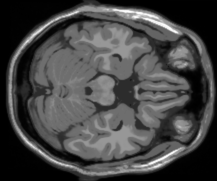
\includegraphics[scale=0.5]{slice_50.png}
			\caption{Slice 50}
	\end{minipage}
\begin{minipage}[bt]{0.3\linewidth}
	\centering
	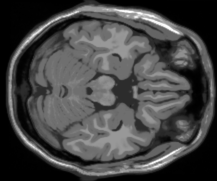
\includegraphics[scale=0.5]{slice_51.png}
	\caption{Slice 51}
\end{minipage}
\begin{minipage}[bt]{0.3\linewidth}
	\centering
	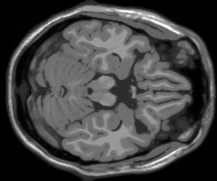
\includegraphics[scale=0.5]{slice_52.png}
	\caption{Slice 52}
\end{minipage}
\end{figure}
\subsection*{Part a}
Here the tomographic reconstruction is performed using the \textbf{Filtered Backprojection} using the \textbf{Ram-Lak} filter. The reconstruction results for slices 50 and 51 are as follows:
\begin{figure}[ht]
	\centering
	\begin{minipage}[bt]{0.5\linewidth}
		\centering
		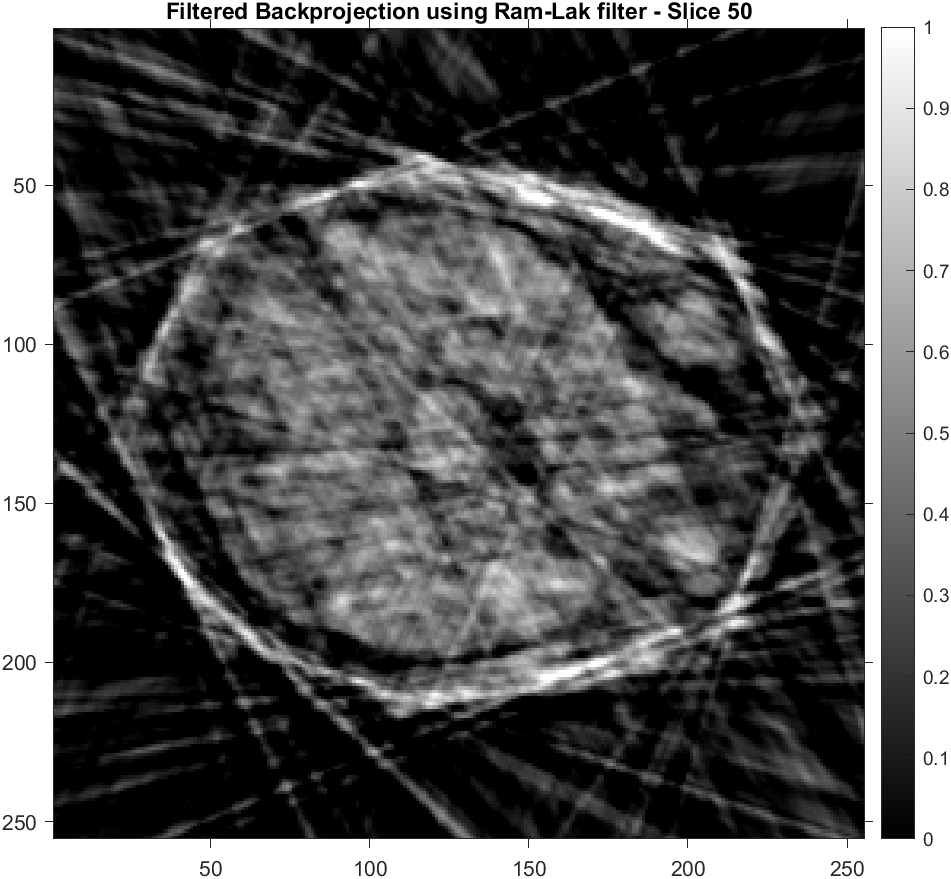
\includegraphics[scale=0.25]{a_50.png}
		\caption{Ram-Lak FBP - Slice 50}
	\end{minipage}
	\begin{minipage}[bt]{0.4\linewidth}
		\centering
		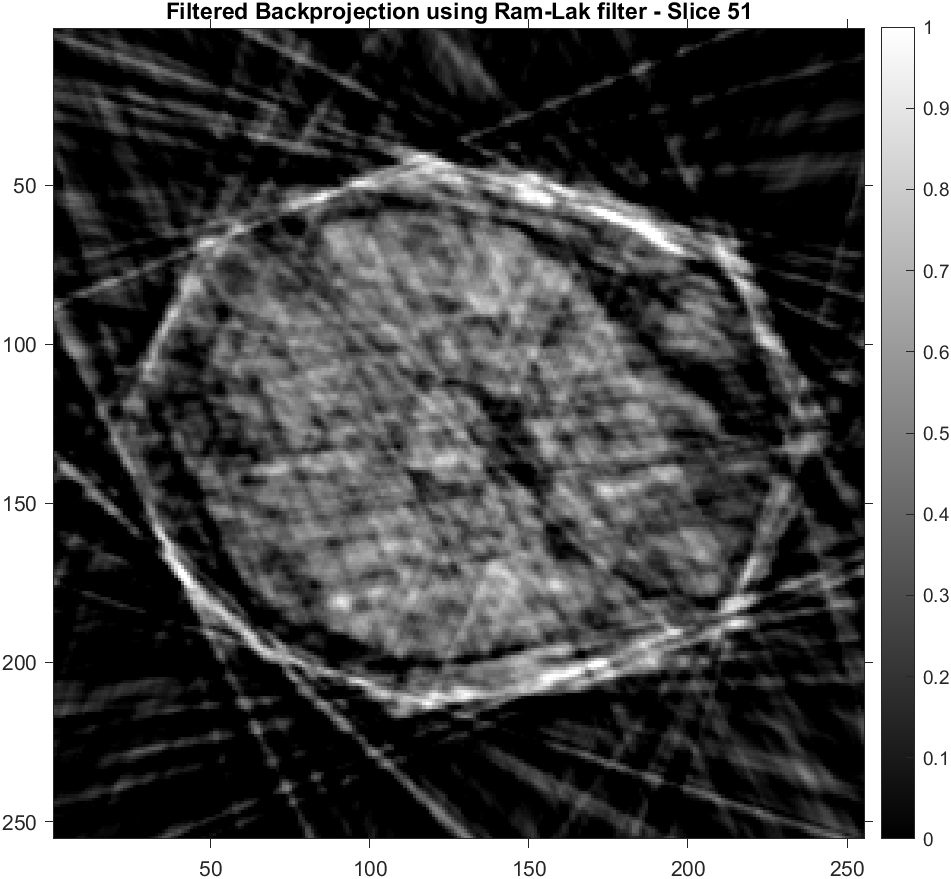
\includegraphics[scale=0.25]{a_51.png}
		\caption{Ram-Lak FBP - Slice 51}
	\end{minipage}
\end{figure}
\subsection*{Part b}
Here the tomographic reconstruction is performed by using the \textbf{Independent Compressive Sensing} based reconstruction for each slice by solving an optimization problem of the form
$$J(x) = \norm{y - Ax}_2^2 + \lambda \norm{x}_1$$
The reconstruction results for slices 50 and 51 are as follows:
\begin{figure}[ht]
	\centering
	\begin{minipage}[bt]{0.5\linewidth}
		\centering
		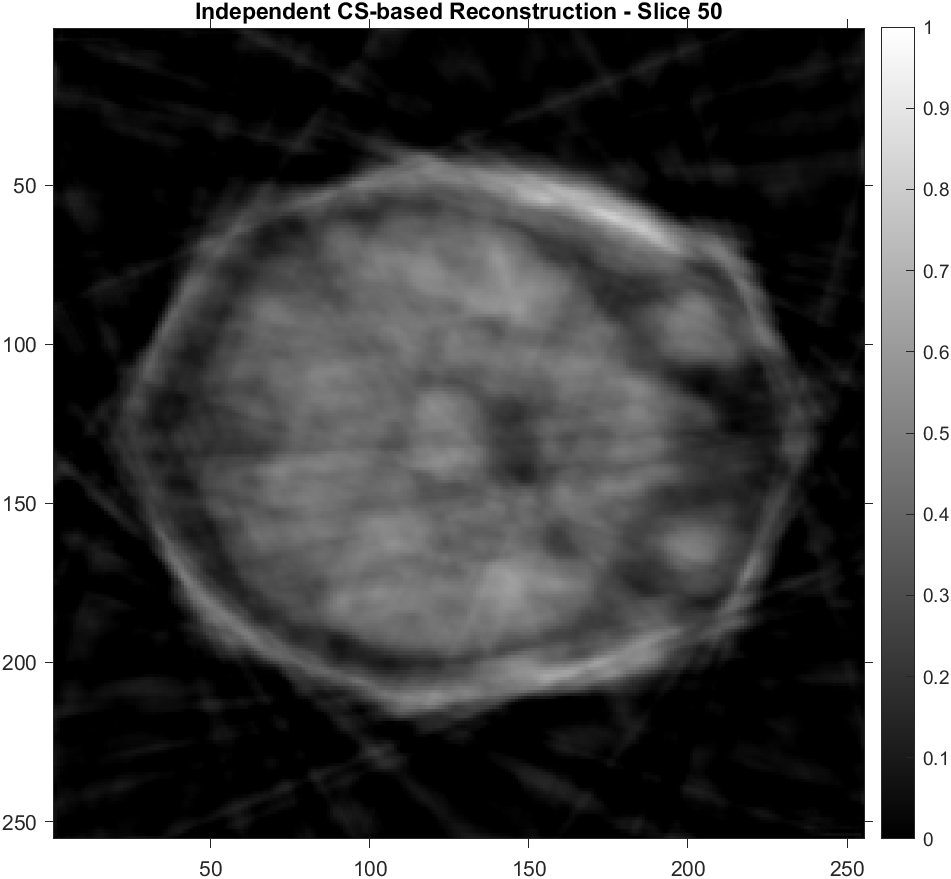
\includegraphics[scale=0.25]{b_50.png}
		\caption{Independent CS - Slice 50}
	\end{minipage}
	\begin{minipage}[bt]{0.4\linewidth}
		\centering
		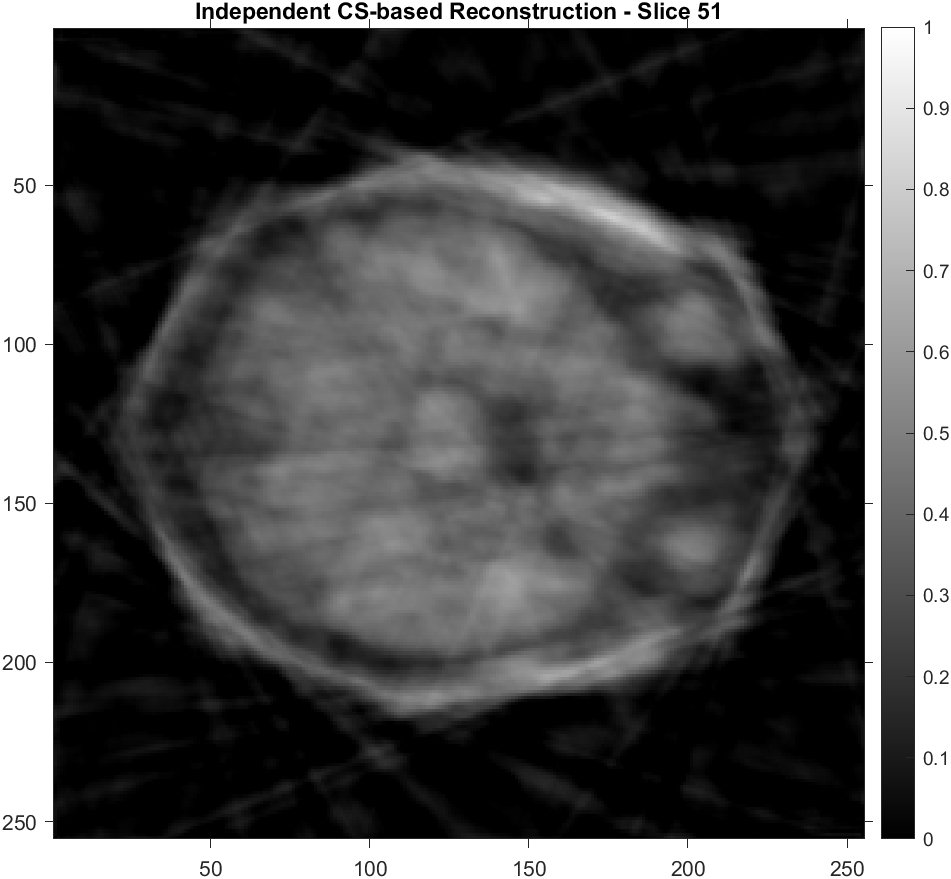
\includegraphics[scale=0.25]{b_51.png}
		\caption{Independent CS - Slice 51}
	\end{minipage}
\end{figure}
\subsection*{Part c}
Here the tomographic reconstruction is performed by using the \textbf{Coupled Compressive Sensing} based reconstruction by solving an optimization problem of the form:
$$J\bigg(\begin{bmatrix}
\beta_1 \\ \Delta \beta_1
\end{bmatrix}\bigg) = \norm{\begin{bmatrix}
	y_1\\y_2
	\end{bmatrix} - \begin{bmatrix}
	R_1U & 0\\
	R_2U & R_2U
	\end{bmatrix} \begin{bmatrix}
	\beta_1 \\ \Delta \beta_1
	\end{bmatrix}}_2^2 + \lambda \norm{\begin{bmatrix}
	\beta_1 \\ \Delta \beta_1
	\end{bmatrix}}_1$$
The reconstruction results for slices 50 and 51 are as follows:
\begin{figure}[ht]
	\centering
	\begin{minipage}[bt]{0.5\linewidth}
		\centering
		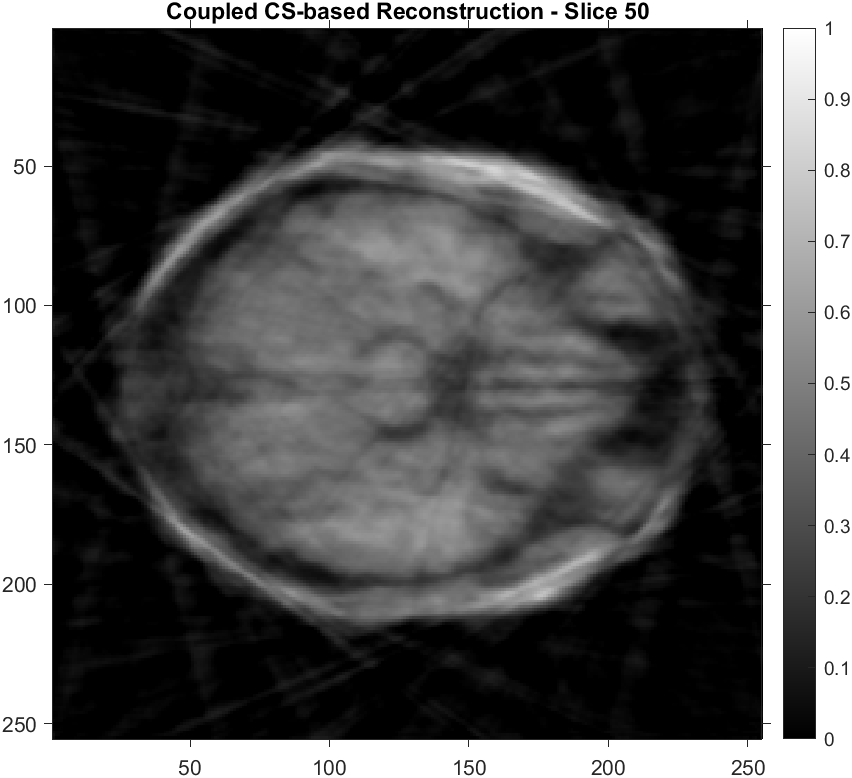
\includegraphics[scale=0.25]{c_50.png}
		\caption{Coupled CS - Slice 50}
	\end{minipage}
	\begin{minipage}[bt]{0.4\linewidth}
		\centering
		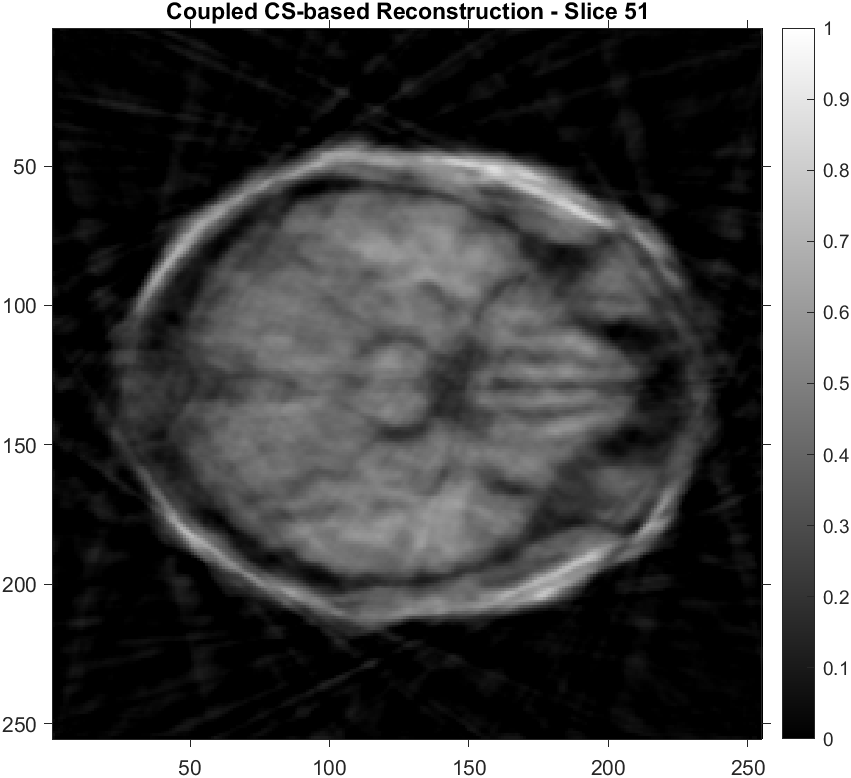
\includegraphics[scale=0.25]{c_51.png}
		\caption{Coupled CS - Slice 51}
	\end{minipage}
\end{figure}
\subsection*{Part d}
Here the tomographic reconstruction is performed by using the \textbf{Coupled Compressive Sensing} based reconstruction \textbf{using 3 slices} by solving an optimization problem of the form:
$$J\bigg(\begin{bmatrix}
\beta_1 \\ \Delta \beta_1 \\ \Delta \beta_2
\end{bmatrix}\bigg) = \norm{\begin{bmatrix}
	y_1\\y_2\\y_3
	\end{bmatrix} - \begin{bmatrix}
	R_1U & 0 & 0\\
	R_2U & R_2U & 0\\
	R_3U & 0 & R_3U
	\end{bmatrix} \begin{bmatrix}
	\beta_1 \\ \Delta \beta_1\\ \Delta \beta_2
	\end{bmatrix}}_2^2 + \lambda \norm{\begin{bmatrix}
	\beta_1 \\ \Delta \beta_1\\ \Delta \beta_2
	\end{bmatrix}}_1$$
\newpage
Here 
\begin{itemize}
 \item  $y_1, y_2, y_3$ are the radon transforms of 3 slices $x_1, x_2, x_3$ under consideration.
 \item $\beta_1$ is the 2D-DCT of first slice $x_1$, vectorized.
  \item $\beta_1 + \Delta \beta_1$ is the 2D-DCT of second slice $x_2$, vectorized.
  \item $\beta_1 + \Delta \beta_2$ is the 2D-DCT of second slice $x_3$, vectorized.
  \item $R_1$ is the radon transform matrix for the random angles used to compute tomographic projections of $x_1$.
  \item $R_2$ is the radon transform matrix for the random angles used to compute tomographic projections of $x_2$.
  \item $R_3$ is the radon transform matrix for the random angles used to compute tomographic projections of $x_3$.
\end{itemize}
The reconstruction results for slices 50, 51 and 52 are as follows:
\begin{figure}[ht]
	\centering
	\begin{minipage}[bt]{0.3\linewidth}
		\centering
		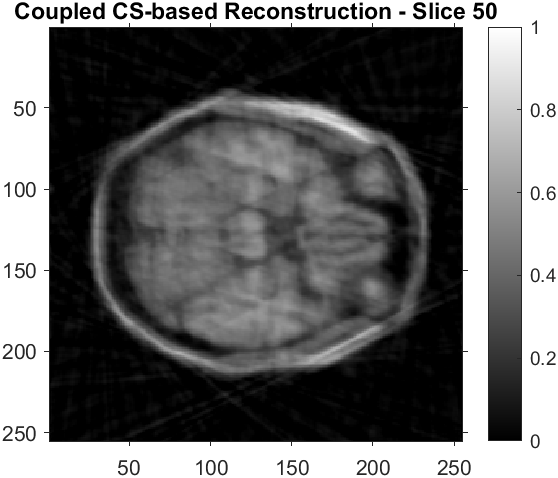
\includegraphics[scale=0.5]{d_50.png}
		\caption{3 CS - Slice 50}
	\end{minipage}
	\begin{minipage}[bt]{0.3\linewidth}
		\centering
		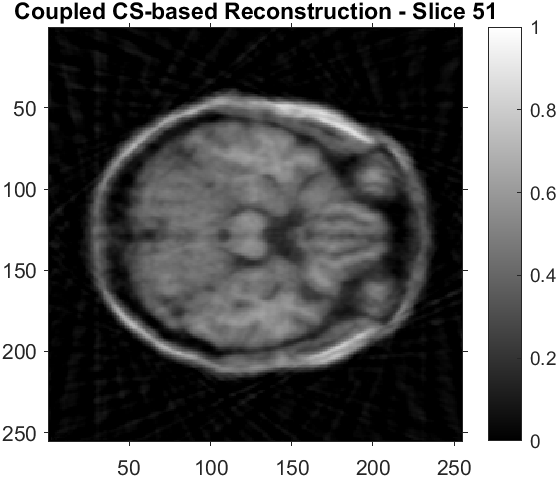
\includegraphics[scale=0.5]{d_51.png}
		\caption{3 CS - Slice 51}
	\end{minipage}
\begin{minipage}[bt]{0.3\linewidth}
	\centering
	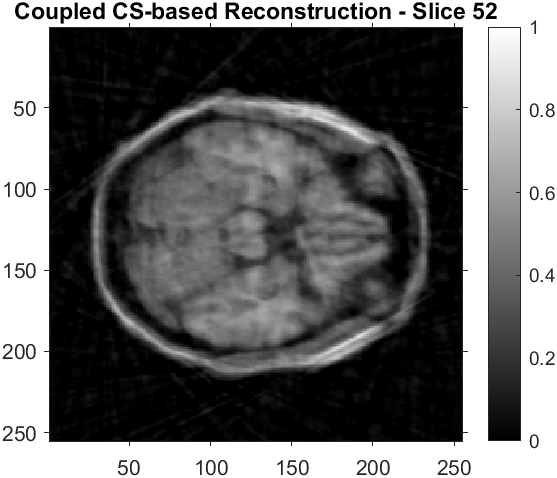
\includegraphics[scale=0.5]{d_52.png}
	\caption{3 CS - Slice 52}
\end{minipage}
\end{figure}
\section*{Question 3}
For the sake of notational simplicity, denote $R(\rho, \theta)$ as the radon transform of $g(x, y)$ at a translation $\rho$ and at an angle $\theta$.
$$R(\rho, \theta) = \int\limits_{-\infty}^\infty \int \limits_{-\infty}^\infty g(x, y) \, \delta(x \cos\theta  + y \sin \theta - \rho)\: dx\,dy$$
\subsection*{Part a}
\begin{eqnarray*}
R\big(g(x-x_0, y-y_0)\big)(\rho, \theta) &=& \int\limits_{-\infty}^\infty \int \limits_{-\infty}^\infty g(x-x_0, y-y_0)\,\delta(x \cos\theta  + y \sin \theta - \rho)\: dx\,dy\\\\
\text{Replace } x \rightarrow u+x_0, y \rightarrow v+y_0&&\\
&=& \int\limits_{-\infty}^\infty \int \limits_{-\infty}^\infty g(u, v)\, \delta\bigg(u\cos \theta + v \sin\theta - \big(\rho - x_0\cos\theta - y_0\sin\theta\big)\bigg)\: dx\,dy\\
&=& R\big(g(u, v)\big)(\rho - x_0\cos\theta - y_0\sin\theta, \theta)\\
&=& R\big(g(x, y)\big)(\rho - x_0\cos\theta - y_0\sin\theta, \theta)
\end{eqnarray*}

\subsection*{Part b}
$$g'(r, \psi) = g(r, \psi - \psi_0)$$
Consider the radon transform in polar coordinates:
$$R(g)(\rho, \theta) = \int \limits_{0}^{2\pi} \int \limits_{0}^\infty g(r, \psi)\, \delta\bigg(r\cos(\psi-\theta) - \rho\bigg)\: r\,dr\,d\psi$$
Now, 
\begin{eqnarray*}
	R(g')(\rho, \theta) &=& \int \limits_{0}^\infty \int \limits_{0}^{2\pi} g'(r, \psi) \: \delta\bigg(r \cos(\psi - \theta) - \rho\bigg) \: r\, dr\, d\psi\\
	&=& \int \limits_{0}^\infty \int \limits_{0}^{2\pi} g(r, \psi - \psi_0) \: \delta\bigg(r \cos(\psi  - \theta) - \rho\bigg) \: r\, dr\, d\psi\\
	\text{Replace }\psi \rightarrow \psi_0 + \alpha &&\\
	&=& \int \limits_0^\infty \int \limits_{-\psi_0}^{2\pi-\psi_0}g(r, \alpha)\, \delta\bigg(r \cos(\alpha + \psi_0 - \theta) - \rho\bigg) \: r\,dr\,d\alpha\\
	&=& \int \limits_0^\infty \int \limits_{0}^{2\pi} g(r, \alpha)\, \delta\bigg(r \cos \big(\alpha - (\theta - \psi_0)\big) - \rho\bigg)\: r \,dr\,d\alpha\\
	\text{Replace } \alpha \rightarrow \psi&&\\
&=&	\int \limits_0^\infty \int \limits_{0}^{2\pi} g(r, \psi)\, \delta\bigg(r \cos \big(\psi - (\theta - \psi_0)\big) - \rho\bigg)\: r \,dr\,d\psi\\
&=& R(g)(\rho, \theta - \psi_0)
\end{eqnarray*}
\subsection*{Part c}
The convolution of two signals $f(x, y)$ and $k(x, y)$ is given by:
$$(f * k)(x, y) = \int \limits_{-\infty}^\infty \int \limits_{-\infty}^\infty f(u, v) k(x-u, y-v)\: dudv$$
The radon transform of the convolution will be
\begin{eqnarray*}
R_\theta(f*k) &=& \int \limits_{-\infty}^\infty \int \limits_{-\infty}^ \infty (f*k)(x, y)\, \delta(x \cos \theta + y \sin \theta - \rho)\: dxdy\\
&=& \int \limits_{-\infty}^\infty \int \limits_{-\infty}^ \infty \int \limits_{-\infty}^\infty \int \limits_{-\infty}^ \infty f(u, v) k(x-u, y-v)\, \delta(x \cos \theta + y \sin \theta - \rho)\: dudv\: dxdy\\
\text{Replace } x-u \rightarrow a, y-v \rightarrow b&&\\
&=& \int \limits_{-\infty}^\infty \int \limits_{-\infty}^ \infty \int \limits_{-\infty}^\infty \int \limits_{-\infty}^ \infty  f(u, v) k(a, b) \, \delta((u+a)\cos\theta + (v+b)\sin \theta - \rho)\: dudv\: dadb\\
&=& \int \limits_{-\infty}^\infty \int \limits_{-\infty}^ \infty \int \limits_{-\infty}^\infty \int \limits_{-\infty}^ \infty f(u, v) k(a, b) \, dudvdadb \int \limits_{-\infty}^\infty \delta(u\cos\theta + v\sin\theta - \sigma)\\
&&\hskip 12em\delta(a\cos\theta + b\sin\theta - (\rho-\sigma))\: d\sigma\\
&=& \int \limits_{-\infty}^\infty \bigg(\int \limits_{-\infty}^\infty\int \limits_{-\infty}^\infty f(u,v) \delta(u\cos\theta + v\sin\theta - \sigma)\, dudv\bigg)\\
&&\bigg(\int \limits_{-\infty}^\infty\int \limits_{-\infty}^\infty k(a, b)\,\delta(a\cos\theta + b\sin\theta - (\rho-\sigma))\,dadb \bigg)\, d\sigma\\
&=&  \int \limits_{-\infty}^\infty R(f)(\sigma, \theta) \, R(k)(\rho - \sigma, \theta)\: d\sigma\\
&=& R_\theta(f) * R_\theta(k)
\end{eqnarray*}
\end{document}
